A 2DEG in a heterojunction is investigated. This chapter is partitioned into two parts. The first part examines the transport properties of a nano-wire for differnet quantum point contacts.\par
The second part presents 2DEG properties of systems of varying geometry. Simulated results are used to explain the interference in an \textsc{Aharonov-Bohm} ring qualitatively by a simple analytical model.\par
\section{Colinear Quantum Point Contacts}
In chapter \ref{sec:conductancefromtransmission} the ``\emph{relation of conductance and transmission}'' \cite{landauer1996} is shown. The transmission of a device with a narrow constriction is \emph{quantized} which has been found by experiments of semiconductor heterojunctions \cite{vanHoutenBeenakker2005} and metals \cite{PhysRevB.36.1284}. The analysis of quantized transmission merits the investigation of small constrictions in more detail.
The two-dimensional electron gas in a semiconductor heterojunction has a \textsc{Fermi} wavelength a hundred times larger than electrons in metal. Due to the large \textsc{Fermi} wavelength the electron transport in mesoscopic devices shows quantization. \emph{Quantum point contacts} are constrictions with a width comparable to the \textsc{Fermi} wavelength of $\lambda_F \approx 30\text{~nm}$ allowing the direct control of the quantization \cite{vanHoutenBeenakker2005}. Due to the large \textsc{Fermi} wavelength these constrictions are \emph{mesoscopic} objects.\par
The quantized nature of the conductance measurements depends on the width of the constriction. Additionally the \emph{potential landscape}, if smooth or abrupt, influences the conductance \cite{PhysRevB.44.8017}.\par
Different potential changes are illustrated in \cref{fig:hardwalled,fig:softwalled,fig:variationalwalled}. \Cref{fig:hardwalled} shows a potential constriction with abrupt walls or \emph{hard walled} potential. This type of potential is found for example in devices etched out of a parent layer via reactive gases or the cleaved edge technique \cite{ApplPhysLett.66.323}. In the adiabatic or soft-walled case the potential landscape varies only slowly in any direction. \Cref{fig:softwalled} illustrates the adiabatic constriction formed of two electrical point charges. A potential which can be varied beween hard and soft walled will be called \emph{variational potential}. A variational potential is designed to investigate the dependence of the conduction on the slope of the constricting potential, see \cref{fig:variationalwalled}. Here the walls can be symmetrically modified to achieve different but constant slopes of the confinement.
\begin{figure}[h!]
\begin{minipage}[c]{0.5\textwidth}
  \begin{tikzpicture}%[every text node part/.style={align=center}]
      \node at (0,0)[above] {\includegraphics[width=0.9\textwidth]{images/qpcrect-crop.png}};
      \axes
\draw[style={<->,thin}] ($1.125*(-1.3,3.6247)$) -- ($1.125*(-0.55,3.25)$) node[midway,left,yshift=-0.5em] {$d$};
\draw[style={<->,thin}] ($1.125*(0,2)$) -- ($1.125*(1,2.5)$) node[midway,above] {$w$};
    \end{tikzpicture}
    \end{minipage}
\begin{minipage}[c]{0.5\textwidth}
 \begin{flalign}\quad\text{Pot}(x,y) =\ &\Theta(d/2-\abs{x})&\notag\\
 \cdot\ &\Theta(\abs{y}-w/2)&\end{flalign}
 \end{minipage}
\caption{Potential landscape of hard-walled quantum point contact. The longitudinal direction of electron flow $x$ and the transverse direction $y$ is denoted. The depth of the wall $d$ the width of the confinement $w$ are illustrated by the arrows. The dimensionless analytical expression of the potential is presented on the right.}\label{fig:hardwalled}
\end{figure}
\begin{figure}[h!]
% \begin{tabularx}{\textwidth}{m{0.45\textwidth} m{0.55\textwidth}}
\begin{minipage}[c]{0.5\textwidth}
  \begin{tikzpicture}%[every text node part/.style={align=center}]
      \node at (0,0)[above] {\includegraphics[width=0.9\textwidth]{images/qpcpoint-crop.png}};
      \axes
\draw[style={<->,thin}] ($1.125*(-1.6,3)$) -- ($1.125*(1.3,4.3)$) node[midway,above] {$w$};
    \end{tikzpicture}
    \end{minipage}
\begin{minipage}[c]{0.5\textwidth}
 \begin{flalign}\quad\text{Pot}(x,y) &= \frac{q}{\sqrt{x^2+(y+w/2)^2}}&\notag\\
 &+\frac{q}{\sqrt{x^2+(y-w/2)^2}}&\end{flalign}
    \end{minipage}
% \end{tabularx}
\caption{Potential landscape of soft-walled quantum point contact of two point charges of charge $q$ and dislocation $w$. The longitudinal direction of electron flow $x$ and the transverse direction $y$ is denoted. The dimensionless analytical expression of the potential is presented on the right.}\label{fig:softwalled}
\end{figure}
% \begin{figure}[h!]
%   \begin{minipage}[c]{0.5\textwidth}
%   \begin{tikzpicture}%[every text node part/.style={align=center}]
%       \node at (0,0)[above] {\includegraphics[width=.9\textwidth]{images/qpcvariational-crop.png}};
%       \axes
% % \draw[style={-,thin}] (2,0.65) -- (2,1.3) node[midway,above] {$w$};
% % \draw [help lines] (0,0) grid (3,3);
%   \coordinate (a) at ($1.125*(1.05,1.62)$);
%   \coordinate (b) at ($1.125*(1.75,2.015)$);
%   % \coordinate (c) at ($(b)+(-0.2,1.322)$);
%   \coordinate (c) at ($1.125*(1.75,3.582)$);
%   \coordinate (d) at ($1.125*(0.21,2.05)$);
%   \coordinate (e) at (0.0506,2.508);
%   \coordinate (f) at (0.73,4.5);
%   \draw[-] (a) node[above,yshift=2em]{$m$} -- (b) node[midway,below,xshift=0.8em]{$\Delta y$} -- (c) --cycle;
%   \draw[dashed] (a) -- (d);
%   \draw[-] (e) -- (f);
%   \draw[dashed] (c) -- (f);
%     \end{tikzpicture}
% \end{minipage}
% \begin{minipage}[c]{0.5\textwidth}
% \begin{flalign}\quad\text{Pot}(x,y) &= e^{-x^2/\xi^2}\cdot\abs{m\cdot y}&\end{flalign} 
% \end{minipage}
% \caption{Example potential landscape of variational-walled quantum point contact used in analysis}\label{fig:variationalwalled}
% \end{figure}
\begin{figure}[h!]
  \begin{minipage}[c]{0.5\textwidth}
  \begin{tikzpicture}%[every text node part/.style={align=center}]
      \node at (0,0)[above] {\includegraphics[width=.9\textwidth]{images/qpcvariational2-crop.png}};
\draw[style={<->,thin}] ($1.125*(-0.205,2)$) -- ($1.125*(0.27,2.25)$) node[midway,above] {$w$};
      \axes
  \coordinate (a) at (1.65,2.3);
  \coordinate (b) at (2.6,2.87825);
  % \coordinate (b) at (2.505,2.81325);
  \coordinate (c) at (2.6,3.982);
  \coordinate (e) at (0.53,2.9);
  \coordinate (f) at (1.45,4.5);
  \draw[-] (a) node[above,xshift=0.5em,yshift=2em]{$m$} -- (b) node[midway,below,yshift=0.3em,xshift=0.8em]{$\Delta y$} -- (c) --cycle;
  \draw[dashed] (a) -- (e);
  \draw[-] (e) -- (f);
  \draw[dashed] (c) -- (f);
    \end{tikzpicture}
\end{minipage}
\begin{minipage}[c]{0.5\textwidth}
\begin{flalign}\quad\text{Pot}(x,y) &= e^{-x^2/\xi^2}\cdot m(\abs{y}- w/2)&\end{flalign} 
\end{minipage}
\caption{Example potential landscape of variational-walled quantum point contact used in analysis. The longitudinal direction of electron flow $x$ and the transverse direction $y$ is denoted. The width at the bottom of the potential $w$ is indicated by arrows. The slope of the transverse confinement $m$ is illustrated by a gradient triangle. The parameter $\xi$ controls the steepness of the walls in $x$ direction. The dimensionless analytical expression of the potential is presented on the right.}\label{fig:variationalwalled}
\end{figure}
The presented quantum point contacts serve only as examples for three classes of constrictions. In the simulations either the geometry of the constriction or the charge of the point charges are varied. Modifying the width of the quantum point contact is usually experimentally achieved by the placement of several gate electrodes either on or in the 2DEG. A negative potential is applied to the electrodes which effectively results in a depopulating of the conductance band in their vicinity. It is important to note that by changing the voltage on the electrodes and therefore the charge not only the width of the potential is changed but also the steepness of the confining potential for a given energy. Hence the transfer from the adiabatic to the diabatic i.e steep walled domain is possible.\par
In the model electrons with a wavevector pointing in the direction of the constriction are placed in the lead at the top of all density plots corresponding to the linear response regime of transport.
For the simulated quantum point contacts the width of the constriction is varied for a fixed energy of $E=0.06\cdot t_0$ corresponding to 15 modes within the unconstriced wire of 200nm width. A lattice spacing a=1 nm, and an effective mass  $m^*=0.026 \times m_0$ as in \cref{sec:validation} are assumed. The \textsc{Rashba} parameter is set to a typical value of $\alpha = 20^{-12}$ eVm\,\cite{Jacob2009Thesis}.
\subsection{Hard-Walled quantum point contacts}
The geometry of quantum devices in 2DEGs prepared by etching commonly exhibits steep walls of the confining potential. Thus the influence of geometrical constrictions on the transport properties of the 2DEG are considered first.
\begin{figure}[h]
\subfloat[]{\label{fig:rectedens}\includegraphics[]{images/238916-wire400x200-Nov-28-2011-17.41edens}}
\subfloat[]{\label{fig:rectspindens}\includegraphics[]{images/238916-wire400x200-Nov-28-2011-17.41spindens}}
\caption{Simulated electron and spin density of a rectangular quantum point contact of  width $w$=100 nm, and depth $d$=60 nm. (a) Two-dimensional electron density. Color code denotes the electron density $n$. (b) Two-dimensional spin density. Color code denotes spin density $s_z$.}
\end{figure}
A constriction similar to the \emph{rectangular} abrupt potential shown in \cref{fig:hardwalled} is used as a starting point of the analysis of 2DEGs with quantum point contacts.\par
The electron density illustrated in \cref{fig:rectedens} shows the expected formation of modes within the constriction. In the areas towards the leads however strong interference disturbs the establishment of continuous electron flux tubes. The interference may be due to backscattering of the propagating electrons. The spin density in \cref{fig:rectspindens} shows a similar interference pattern as the electron density. Interestingly two areas of dominant upward polarization to the left and downward polarization to the right side of the constriction is present. This effect seems related to the diffusion of spin injection from the quantum point contact into the lead.\par
\begin{figure}[h]
\centering
\includegraphics[]{images/238916-wire400x200-Nov-28-2011-17.41trans}
\caption{Simulated transmission profile}
\end{figure}
In the conductance distinct steps of height 2~$e^2/h$ are visible. In each step the conductance increases by one conductance quantum $e^2/h$ per mode per spin-up and spin-down electron.\par
\begin{figure}[h]
\subfloat[]{\label{fig:triedens}\includegraphics[]{images/wire400x200-Nov-28-2011-00.47edens}}
\subfloat[]{\label{fig:trispindens}\includegraphics[]{images/wire400x200-Nov-28-2011-00.47spindens}}
\caption{Simulated electron and spin density for triangle shaped constriction tip. Snapshot corresponds to a a width of $w=$100nm}
\end{figure}
To remedy the abrupt potential change a \emph{triangular} potential is introduced. This geometry comes close to the physical shape of the constriction used by \textsc{Wees} et. al \cite{PhysRevLett.60.848}. Due to the less abrupt potential in the $x$ and $y$ direction the electron flow shows more continuous densities in \cref{fig:triedens}. There also appear a number of points of high electron density in the upper and lower part due to the reflections on the perpendicular quantum point contact wall.\par
\begin{figure}[h]
\centering
\includegraphics[]{images/wire400x200-Nov-28-2011-00.47trans}
\caption{Simulated transmission profile in dependence of the quantum point contact width}\label{fig:tritrans}
\end{figure}
In the spin density plot in \cref{fig:trispindens} a spin split pattern very similar to the rectangular case can be observed. The spin-down electrons and spin-up electrons will be separated after passing the constriction. The interference pattern along the central axis in $y$ direction of the wire is more complex than in the rectangular case in \cref{fig:rectspindens}. Additionally the almost parallel spin split in the very ends of the device is diminished. These effects might explain the unexpected result of the conductance quantization or the lack thereof.
It is interesting to note that there are almost no steps visible in \cref{fig:tritrans} although the potential is more adiabatic because of the angled change in $x$ direction. This can be seen by the continuous lines of electron density within the constriction in \cref{fig:triedens}. For low intrusion of the quantum point contact tips smooth steps of height 2 $e^2/h$ are observed. A smoother shape of the steps is expected for devices with less abrupt changes but the tips still present \emph{infinite} walls. A possible non-physical cause might lie in the discretization. Because the device is mapped on a square lattice the angled walls of the constriction become highly ragged. This series of longitudinal and transverse wall segments might give rise to a steep increase of scattering effectively smoothing out the conductance steps due to a higher spread in the kinetic energy distribution of the propagating electrons.
% \begin{figure}[h]
% \subfloat[Edens]{\includegraphics[]{images/}}
% \subfloat[Spindens]{\includegraphics[]{images/}}
% \caption{Simulated electron and spin density}
% \end{figure}
% \begin{figure}[h]
% \centering
% \includegraphics[]{images/}
% \caption{Simulated transmission profile}
% \end{figure}
\FloatBarrier
\subsection{Soft-Walled Quantum Point Contacts}
The geometrical shape of the constriction influences the transport properties of the device as seen in the previous section. Changing the geometry perpendicular to the $z$-axis smoothed out most features related to quantized conductance either physically or by introducing artificial complexity not found in the actual continuous system.\par
One possible remedy is to alter the slope of the confining potential landscape perpendicular to the $x$ and $y$-axis. This stands in opposition to the infinite slope of the hard walled potentials considered before. A potential wall slowly varying in respect to the $x$ and $y$ coordinates will be called \emph{soft walled}.\par
\begin{figure}[h]
\subfloat[Electron density $n$]{\label{fig:sphericaledens}\includegraphics[]{images/wire400x200-Nov-27-2011-21.41edens}}
\subfloat[Spin density in measures of $\hbar/m^2$]{\label{fig:sphericalspindens}\includegraphics[]{images/wire400x200-Nov-27-2011-21.41spindens}}
\caption{Simulated electron and spin density of a 2DEG with spherical constriction.}
\end{figure}
The \emph{spherical} electrode tip has a shape with characteristics of both the abrupt and adiabatically varying potential walls. The hard walls perpendicular to each lateral axis are gradually smoothed towards higher potential. The rectangular or triangular tip of the gate electrodes are replaced by a quarter-circle which for small intrusions mimics the potential introduced by a top gate above the 2DEG. Looking at the electron density in \cref{fig:sphericaledens} a resemblance to the prior tip shapes can be seen. The structure exhibits increased continuous electron densities as well as points of high electron densities symmetrically arranged in the upper and lower half similar to the triangular tip. Also the spin densities in \cref{fig:sphericalspindens} only differ slightly from the triangular case.\par
\begin{figure}[h]
\centering
\includegraphics[]{images/wire400x200-Nov-27-2011-21.41trans}
\caption{Simulated transmission profile}
\end{figure}
Despite the similarities to the triangular case clearly pronounced steps are seen in the conductance profile. The variations near the steps are smoothed out without the loss of discrete steps of height 2 $e^2/h$. Because of these characteristics the spherical potential is used to validate the results of the conductance calculations in section \ref{sec:validation}.\par
\begin{figure}[h]
\subfloat[Electron density $n$ for the 2DEG constrained in the $y$ direction by two point charges.]{\label{fig:pointedens}\includegraphics[]{images/242255-wire400x200-Dec-02-2011-23.08edens}}
\subfloat[Spin density $s_z$ of the 2DEG constrained in the $y$ direction by two point charges.]{\label{fig:pointspindens}\includegraphics[]{images/242255-wire400x200-Dec-02-2011-23.08spindens}}
\caption{Simulated electron and spin density for a constriction formed by two point charges c.f.~\cref{fig:softwalled}. The point charges are located at the transverse boundary of the wire 200nm apart. Snapshot corresponds to $q\approx 1.5\cdot 10^{-18}$ C}
\end{figure}
In the following simulation point charges are introduced in the vicinity of the 2DEG to model a constriction formed by gate electrodes more closely. A quantum point contact of this kind exhibits a very slow varying potential throughout large parts with almost infinite slopes near the location $r_q$ of the point charges due to the $\sim 1/r_q$ dependency.\par
The electron density illustrated in \cref{fig:pointedens} show the expected continuous flux tube at the very edge of the nanowire while the center region is subject to complex interference. An interference pattern can also be observed before and after the quantum point contact. The pattern is much simpler in comparison to all prior quantum point contacts. The lateral offset near the upper and lower lead are due to the necessity to cut off the potential at some point which would otherwise extend to infinity.
Although the maximum spin splitting is lower compared to all prior quantum point contacts it exhibits a much simplified interference pattern with localized areas of maximum polarization and otherwise almost negligible polarization. The simplicity of the pattern is due to the reduced number of modes. The probability distribution of the electrons is laterally confined to the same area. Due to the slow decrease of the potential there exists a finite potential throughout the device.\par
\begin{figure}[h]
\centering
\includegraphics[]{images/242255-wire400x200-Dec-02-2011-23.08trans}
\caption{Simulated transmission profile of quantum point contact of two point charges for a spin degenerate system}\label{fig:qpcpointnospin}
\end{figure}
In \cref{fig:pointtrans} the conductance profile mirrors both, the hard and the soft walled contributions to the potential. A well pronounced first and second conductance step can be observed but the steps smooth out more with decreasing charge. Interestingly the steps become well pronounced again when the charge approaches zero. As this pattern is also observed for spin degenerate systems as can be observed in \cref{fig:qpcpointnospin} a relation of this effect to a spin-orbit coupling seems unlikely. 
The disappearance of steps can be explained by the onset of \emph{inter-subband scattering} which have been found to have significant effect starting at the fourth mode \cite{Lehmann2011}. If inter-subband scattering is indeed the cause for the smoothing of the conductance profile the re-appearance of noticeable steps would correspond to the reduction of inter-subband scattering due to some change in the device at lower charge.
Note that as the charge decreases the steepness of the potential increases for a given electron energy $E_{e^-}$ as illustrated in \cref{fig:differentq}.
The only obvious change in the 2DEG at lower charge is the height and steepness of the potential landscape. To investigate the relation of the steepness of the potential landscape to the diminishing conductance quantization a parametrized  quantum point contact is introduced into the 2DEG, see \cref{fig:variationalwalled}.
\begin{figure}[h] 
\centering
\subfloat[Simulated conductance profile in dependence of quantum point contact width.]{\includegraphics[]{images/242368-wire400x200-Dec-03-2011-04.35trans}}
\subfloat[Transverse potential profile in Volt at different charge $q_1 = 6.5 \cdot 10^{-18}$C and $q_2= 1 \cdot 10^{-18}$C.]{\label{fig:differentq}\includegraphics{images/differentq}}
\caption{Conductance profile and sample of confining potential at different charge.}\label{fig:pointtrans}
\end{figure}
\FloatBarrier
\subsection{Variational-Walled Quantum Point Contacts}
The effects of  the wall slope on the smoothness of the conductance profile and thus possibly on the inter-subband scattering are investigated by increasing the width of the constriction for many different slopes $m$. Above a slope of $m \approx 0.03$ the conduction shows quantized steps with no significant influences if the slope changes in that interval. For slowly varying potential slopes a noticeable change in conduction quantization can be observed, see \cref{fig:slopes}. \Cref{fig:conductances} shows conductance profiles at constant slopes. A significant change in quantization is only observed in the slope interval $0.008 < m < 0.032$.\par
The electron densities in \cref{fig:variedens1} and \cref{fig:variedens2} provide further indications of inter-subband scattering. The comparison of both figures shows that the electron density for the softer quantum point contact is much less localized in discrete channels. This could indicate an increase in interaction of the modes passing through the quantum point contact.\par
\begin{figure}[h] 
\centering
\subfloat[Conductance profiles for different slopes $m$]{\label{fig:slope_cuts}\includegraphics[]{images/slope_cuts.pdf}}
\subfloat[Full conductance profile for quantum point contact opening sweep. Plotted is the conductance of the quantum point contact for different width $w$ and transverse steepness $m$ of the constriction]{\label{fig:slopes}\includegraphics[width=0.5\textwidth]{images/slopes.png}}
\caption{Conductance profiles at different slopes and full conduction profile slope vs. width.}\label{fig:conductances}
\end{figure}
Interestingly the spin split is increased for the smoother walled quantum point contact in \cref{fig:varispindens1} in comparison to \cref{fig:varispindens2,fig:trispindens,fig:rectspindens,fig:pointspindens}. Additionally the spin plit exhibits less dominant interference than any hard walled potential since the smoother the potential landscape the less likely is a reflection that alters the electron propagation.\par
There seem to be strong indications for the interaction of wall slope and possible inter-subband scattering similar to the mixing of intra-subband eigenstates due to higher order effects of the \textsc{Rashba} spin-orbit interaction \cite{Wolfgang2003PhysicaE.18.337}. Spin-orbit coupling that is influenced by the shape of the constriction could also explain the difference in spin-polarization and could be subject to further analysis.
\begin{figure}[h]
\subfloat[Electron density $n$ for the 2DEG.]{\label{fig:variedens1}\includegraphics[]{images/1edens}}
\subfloat[Spin density $s_z$ of the 2DEG.]{\label{fig:varispindens1}\includegraphics[]{images/1spindens}}
\caption{Simulated electron and spin density for a constriction formed by a variational-walled constriction of slope $m=0.008$. Snapshot corresponds to a conductance of 16$e^2/h$}
\end{figure}
\begin{figure}[h]
\subfloat[Electron density $n$ for the 2DEG.]{\label{fig:variedens2}\includegraphics[]{images/4edens}}
\subfloat[Spin density $s_z$ of the 2DEG.]{\label{fig:varispindens2}\includegraphics[]{images/4spindens}}
\caption{Simulated electron and spin density for a constriction formed by a variational-walled constriction of slope $m=0.032$. Snapshot corresponds to a conductance of 16 $e^2/h$ }
\end{figure}
\FloatBarrier
\section{Non-Colinear devices}
The geometry of the device can be changed to induce a break of the symmetry of the spin split. To that end the assumption of colinear leads has to be dropped.
\subsection{Curved Nanowire}
A simple bend in the nanowire already introduces complex interactions in real-space as well as spin-space. This is demonstrated in \cref{fig:curvedens1,fig:curvedens2,fig:curvedens3,fig:curvspindens1,fig:curvspindens2,fig:curvspindens3}. The first three modes correspond respectively to the energies 0.003eV, 0.036eV and 0.081eV of a straight nanowire of same width. If compared to \cref{fig:dens1,fig:dens2,fig:dens3} for example an apparent change is immeadiatlely seen. The spacial distribution of electrons along the wire is not constant and the spin densities exhibit a preference for up polarized electrons. Note that the scales change about the order of two to prevent the loss of details for smaller spin split and electron densities. The features of the curved 2DEG are energy dependent. For all three modes the spin-down density is suppressed. For the third mode the spin density shows an irregular interference pattern.\par
\begin{figure}[h!]
\subfloat[Electron density of first mode in curved nano-wire. $E_{mode}=0.003$eV.]{\label{fig:curvedens1}\includegraphics[]{images/curve_1modes_edens}}
\subfloat[Electron density of second mode in curved nano-wire. $E_{mode}=0.036$eV.]{\label{fig:curvedens2}\includegraphics[]{images/curve_2modes_edens}}
\subfloat[Electron density of third mode in curved nano-wire. $E_{mode}=0.081$eV. ]{\label{fig:curvedens3}\includegraphics[]{images/curve_3modes_edens}}
\caption{Electron densities for a curved nano-wire of 40nm width. Because of the bend the wire-width is marginally reduced in the curve. Colour indicates electron density. The density increases from Blue=0 to Red=Max($n$).}
\end{figure}
\begin{figure}[h!]
\subfloat[Spin density of first mode in curved nano-wire.  $E_{mode}=0.003$eV.]{\label{fig:curvspindens1}\includegraphics[]{images/curve_1modes_spindens}}
\subfloat[Spin density of second mode in curved nano-wire. $E_{mode}=0.036$eV.]{\label{fig:curvspindens2}\includegraphics[]{images/curve_2modes_spindens}}
\subfloat[Spin density of third mode in curved nano-wire. $E_{mode}=0.081$eV.]{\label{fig:curvspindens3}\includegraphics[]{images/curve_3modes_spindens}}
\caption{Spin densities for a curved nano-wire of 40nm width. Because of the bend the wire-width is marginally reduced in the curve. Colours indicate spin polarization. Red=Up, Blue=Down.}
\end{figure}
\subsection{\textsc{Aharonov-Bohm} Ring Interferometer}
An interferometer is a common approach to the manipulation of properties of wave objects. A simple realization of such an interferometer is given by a modification of the \textsc{Arahonov-Bohm} ring. The \textsc{Arahonov-Bohm} ring is a two-dimensional annulus where the difference of inner and outer radius that is maller than the inner radius $\abs{r_o- r_i} \ll r_i$, see \cref{fig:aharonovbohmring}. 
Spin interference has been achieved via the attachment of multiple leads \cite{PhysRevB.75.035304} or the application of an electro-magnetic field \cite{PhysRevB.69.155335} to the \textsc{Arahonov-Bohm} ring.\par
\begin{figure}[!h]
\centering
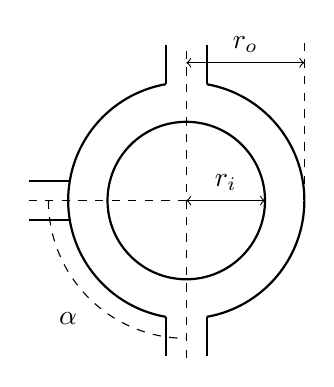
\begin{tikzpicture}
  % \draw[step=.5cm,gray,very thin] (-2,-2) grid (2,2);
  % \draw[dashed] (1.5,0) -- (1.5,0);
  \draw[dashed] (0,-2) -- (0,2);
  \draw[dashed] (0,-2) -- (0,2);
  \draw[dashed] (0,0) -- (-2,0);
  % \draw[dashed] (1,0) -- ++(0,1.5);
  \draw[dashed] (1.5,0) -- ++(0,2);
  \draw[<->] (0,1.75) -- node[above] {$r_o$}++(1.5,0);
  \draw[<->] (0,0) -- node[above] {$r_i$}++(1,0);
  \draw[dashed] (-1.75,0) arc (0:90:-1.75);
  \node (a) at (-1.5,-1.5) {$\alpha$};
  \draw[thick] (0,0) circle (1);
  \draw[thick] (1.5,0) arc (0:80:1.5) coordinate (n1);
  \draw[thick] (-1.5,0) arc (0:-80:-1.5) coordinate (n2);
  \draw[thick] (n1)-- ++(0,0.5);
  \draw[thick] (n2)-- ++(0,0.5);
  \draw[thick] (1.5,0) arc (0:-80:1.5) coordinate (n3);
  \draw[thick] (-1.5,0) arc (0:80:-1.5) coordinate (n4);
  \draw[thick] (n3)-- ++(0,-0.5);
  \draw[thick] (n4)-- ++(0,-0.5);
  \draw[thick] (-2,0.25)-- ++(0.51,0);
  \draw[thick] (-2,-0.25)-- ++(0.51,0);
\end{tikzpicture}
\caption{\textsc{Aharonov-Bohm} ring based interferometer of inner radius $r_i=65$~nm and outer radius $r_o=75$~nm. The angle $\alpha$ denotes the rotation of the lower lead to the upper lead. Here $\alpha=\pi/2$}\label{fig:aharonovbohmring}
\end{figure}
The most basic interferometer is obtained by the attachment to of two leads to the \textsc{Aharonov-Bohm} ring. To investigate changes in spin properties of the 2DEG one of the leads is then rotated against the other to obtain different enclosed angles. The device and process is sketched in \cref{fig:aharonovbohmring}.
\begin{figure}[h!]
\subfloat[Electron density $n$. Enclosing angle $\alpha=0$.]{\label{fig:ring0edens}\includegraphics[]{images/ring0edens}}
\subfloat[Electron density $n$. Enclosing angle $\alpha=\pi/2$.]{\label{fig:ring90edens}\includegraphics[]{images/ring90edens}}
\subfloat[Electron density $n$. Enclosing angle $\alpha=-\pi/2$.]{\label{fig:ringneg90edens}\includegraphics[]{images/ringneg90edens}}
\caption{Electron densities in \textsc{Aharonov-Bohm} type ring for three different enclosing angles. Color denotes density, Blue=0, Red=Max($n$).} 
\end{figure}
\begin{figure}[h!]
\subfloat[Spin density $s_z$. Enclosing angle $\alpha=0$.]{\label{fig:ring0spindens}\includegraphics[]{images/ring0spindens}}
\subfloat[Spin density $s_z$. Enclosing angle $\alpha=\pi/2$.]{\label{fig:ring90spindens}\includegraphics[]{images/ring90spindens}}
\subfloat[Spin density $s_z$. Enclosing angle $\alpha=-\pi/2$]{\label{fig:ringneg90spindens}\includegraphics[]{images/ringneg90spindens}}
\caption{Spin densities in \textsc{Aharonov-Bohm} type ring for three different enclosing angles. Color denotes spin polarization. Blue=Down, Red=Up}
\end{figure}
Already for colinear leads the interference of spin is well pronounced. In contrast to a wire or closed ring \cite{PhysRevB.82.165322} the polarization depends on the angular coordinate $\phi$.
The spins interact to form a standing wave in steady state. The circumference of a concentric circle in the center of inner and outer circle is $c\approx 408$~nm. For the energy $E=0.068$~eV 23 peaks and troughs of the standing wave can be observed which corresponds to a wavelength of $\lambda_{\text{spin}}=17.75$~nm. This length is well below the spin-precession length in undisturbed geometries of $L_{SO}\approx230$~nm due to the strength of the \textsc{Rashba} spin-orbit interaction $\alpha_{RSO}$ considered.\par
Upon rotation of the lower lead the interference pattern changes considerably in amplitude and spatial profile. The phase of the standing wave appears to be fixed to the bottom lead and rotates the peaks and troughs according to the angle the lead has been rotated. Whereas the polarization in the leads is almost negligible throughout \cref{fig:ring0edens,fig:ring90edens,fig:ringneg90edens,fig:ring0spindens,fig:ring90spindens,fig:ringneg90spindens} the amplitude increases sharply within the ring. The amplitudes of spin polarization within the \textsc{Aharonov-Bohm} ring with rotated lead decrease gradually with increasing rotation in about one order of magnitude.\par
For the presented angles of 0,$\pi/2$ and $-\pi/2$ three very distinct situations occur. While the spin up to spin down amplitude ratio is unity for the symmetric device in \cref{fig:ring0edens} it reaches $n_{\uparrow}/n_{\downarrow}=5$ for $\alpha=\pi/2$ rotation in \cref{fig:ring90edens} and $n_{\uparrow}/n_{\downarrow}=0.2$ for $\alpha=-\pi/2$ rotation in \cref{fig:ringneg90spindens}. The electron densities in the ring with rotated leads are about twice as large in the longer arms than the shorter arms what is probably at least in part correlated to the increase in spin density.\par
Qualitatively this result is reproduced analytically for a one dimensional ring for the presented rotations. Solving the \hamil{} for closed ring in polar coordinates one obtains the four eigenstates in each arm \cite{nitta1999.695}:
\begin{align}
\Psi^{\pm}_{\uparrow} = e^{i\phi}\begin{pmatrix}\text{cos}(\theta/2)\\\pm\text{sin}(\theta/2)e^{i\phi}\end{pmatrix} 
\qquad\text{and}\qquad
\Psi^{\pm}_{\downarrow} = e^{\pm i\phi}\begin{pmatrix}\pm\text{sin}(\theta/2)e^{-i\phi}\\-\text{cos}(\theta/2)\end{pmatrix}
\end{align}
Plus and minus denotes the direction of travel and $\uparrow,\downarrow$ spin up and spin down respectively. Expanding each wave function in terms of the eigenstates the interference pattern in \cref{fig:ring90spindens} can be reproduced assuming partial reflection of the spin-up wave function and total transmission of the-spin down wave function at the junctions in the right arm and partial reflection of both spin states at the junctions in the left arm. 
\begin{figure}[!h]
\centering
\includegraphics[scale=0.5]{images/spinors}
\caption{Expansion of spin states in eigenstates of the closed ring. Negative $\phi$ corresponds to the left arm and positive $\phi$ to the right.}
\end{figure}
This model breaks down for arbitrary enclosing angles as the coupling to the leads becomes significant. Due to the coupling of spin states to the lead the eigenstates of the isolated ring do not give an accurate model of the physical situation.
